\documentclass[11pt]{article}
\usepackage{fullpage}

% \usepackage[backref=true]{biblatex}

\usepackage{amsmath,amssymb,amsthm}
\usepackage{graphicx}
\usepackage{hyperref}	


\DeclareMathOperator{\vol}{Vol}
\DeclareMathOperator{\kNN}{kNN}
\DeclareMathOperator{\NN}{NN}


\title{Exact Computation of a Manifold Metric, via Shortest Paths on a
graph}
\author{
  Timothy Chu \\
  CMU\\
  \texttt{tzchu@andrew.cmu.edu}
  \and
  Gary L.\ Miller\\
  CMU\\
  \texttt{glmiller@cs.cmu.edu} \\
  \and
    \newline
  Donald Sheehy\\
  University of Connecticut \\
  \texttt{don.r.sheehy@gmail.com}
}
	
\newcommand{\e}{\varepsilon}
\newcommand{\eps}{\varepsilon}
\newcommand{\volt}{\overrightarrow{v}}
\newcommand{\EE}{\textbf{E}}
\newcommand{\LGinv}{L_G^\dag}
\newcommand{\inv}{(\LGinv)^{1/2}}
\newcommand{\Br}{\overline{B}}
\newcommand{\vr}{\overline{v}}
\newcommand{\xr}{\overline{x}}
\newcommand{\pr}{\overline{p}}
\newcommand{\Rr}{\overline{R}}
\newcommand{\Gr}{\overline{G}}
\newcommand{\Conv}{\mathcal{C}}
\newcommand{\Convr}{\overline{\mathcal{C}}}
\newcommand{\g}{\textbf{g}}
\newcommand{\B}{\mathbb{B}}

\newcommand{\len}{\ell}
\newcommand{\R}{\mathbb{R}}
\newcommand{\ourpath}{\mathrm{path}}
\newcommand{\dist}{\mathbf{d}}
\newcommand{\distto}{\mathbf{r}}
\renewcommand{\because}[1]{&\left[\text{\small{#1}}\right]}

\newtheorem{claim}{Claim}
\newtheorem{observation}{Observation}
\newtheorem{problem}{Problem}
\newtheorem{theorem}{Theorem}[section]
\newtheorem{prop}[theorem]{Proposition}
\newtheorem{corollary}{Corollary}[theorem]
\newtheorem{remark}{Remark}[theorem]
\newtheorem{lemma}[theorem]{Lemma}
\newtheorem{definition}[theorem]{Definition}

\usepackage{color}

\newcommand{\gary}[1]{{\bf \color{red} Gary: #1}}
%\newcommand{\gary}[1]{}
\newcommand{\tim}[1]{{\bf \color{red} Tim: #1}}
%\newcommand{\tim}[1]{}
\newcommand{\don}[1]{{\bf \color{red} Don: #1}}
%\newcommand{\don}[1]{}

\begin{document}

  \setcounter{page}{0}
  \maketitle
  \thispagestyle{empty}
  \begin{abstract}

  % Basic Object and main result
  Data-sensitive metrics adapt distances locally based the density of data points with the goal of aligning distances and some notion of similarity.
  In this paper, we give the first exact algorithm for computing a data-sensitive metric called the Nearest Neighbor Metric.
  In fact, we prove the surprising result that a previously published $3$-approximation is an exact algorithm.

  % Surprising and Hard
  The Nearest Neighbor Metric can be viewed as a special case of a density-based distance used in machine learning, or it can be seen as an example of a manifold metric.
  Previous computational research on such metrics despaired of computing exact distances on account of the apparent difficulty of minimizing over all continuous paths between a pair of points.

  % ancillary results
  We leverage the exact computation of the Nearest Neighbor Metric to compute sparse spanners and persistent homology.
  We also explore the behavior of the metric built from point sets drawn from an underlying distribution and consider the more general case of inputs that are countable collections of compact sets.

  % Interesting Connections
  The main results connect several classical theories such as the conformal change of Riemannian metrics and the screw theory of Schoenberg and Von Neumann.
  We also develop some novel proof techniques based on the combination of screw functions and Lipschitz extensions that may be of independent interest.

\end{abstract}

  \clearpage
  
  %  \input{old_introduction}
  \section{Introduction} A foundational hypothesis in non-linear dimension
reduction and machine learning is that data can be represented as points in
Euclidean space, and appropriate metrics on these points can be generated
to solve a variety of problems including clustering, classification,
regression, surface reconstruction, topological property inference, and
more. In machine learning, two data points should intuitively be considered
close if they are in the same data cluster, even if their Euclidean
distance is far. This property is called the \textbf{density-sensitive}
property.\gary{Use data-sensitive instead of density-sensitive}

Density-sensitive metrics are considered fundamental in the study of
machine learning, and are implicitly central in celebrated machine learning
methods such as $k$-NN graph methods, manifold learning, level-set methods,
single-linkage clustering, and Euclidean MST-based clustering (See Appendix
~\ref{} for details). The construction of appropriate density-sensitive
metrics is an active area of research in machine learning. We consider a
simple density-sensitive metric with an underlying manifold structure.
This metric is called the Nearest Neighbor Metric, and it and its close
variants have been studied in the past by multiple researchers. 
In this paper, we show how to
compute the Nearest Neighbor metric exactly for any dimension, which solves
one of the most important and challenging problem for any manifold-based
metric.

To define the nearest neighbor metric, we first define the notion of a
density-based distance. This is a slight variation of the original
definition from~\cite{}.

\begin{definition}
Given a continuous cost function $c:\R^k \rightarrow \R$, we define the density-based
cost of a path $\gamma$ relative to $c$ as: 
\[ \len_c(\gamma) = \int_{0}^1 c(\gamma(t)) \| \gamma'(t) \|dt. \]
Here, the path $\gamma$ is defined as a continuous mapping $\gamma:[0,1]
\to \R^k$.
Let $\ourpath(a,b)$ denote the set
of piecewise-$C_1$ paths from $a$ to $b$.  We will compute the
lengths of paths relative to the distance function $\distto_p$ as
follows. 
We then define the \textbf{density-based distance} between two points $a, b \in
\R^k$ as 
\[ d_c(a,b) \inf_{\gamma\in\ourpath(a,b)} \len_c(\gamma)\]
\end{definition}

\begin{figure}[htbp]
  \centering
    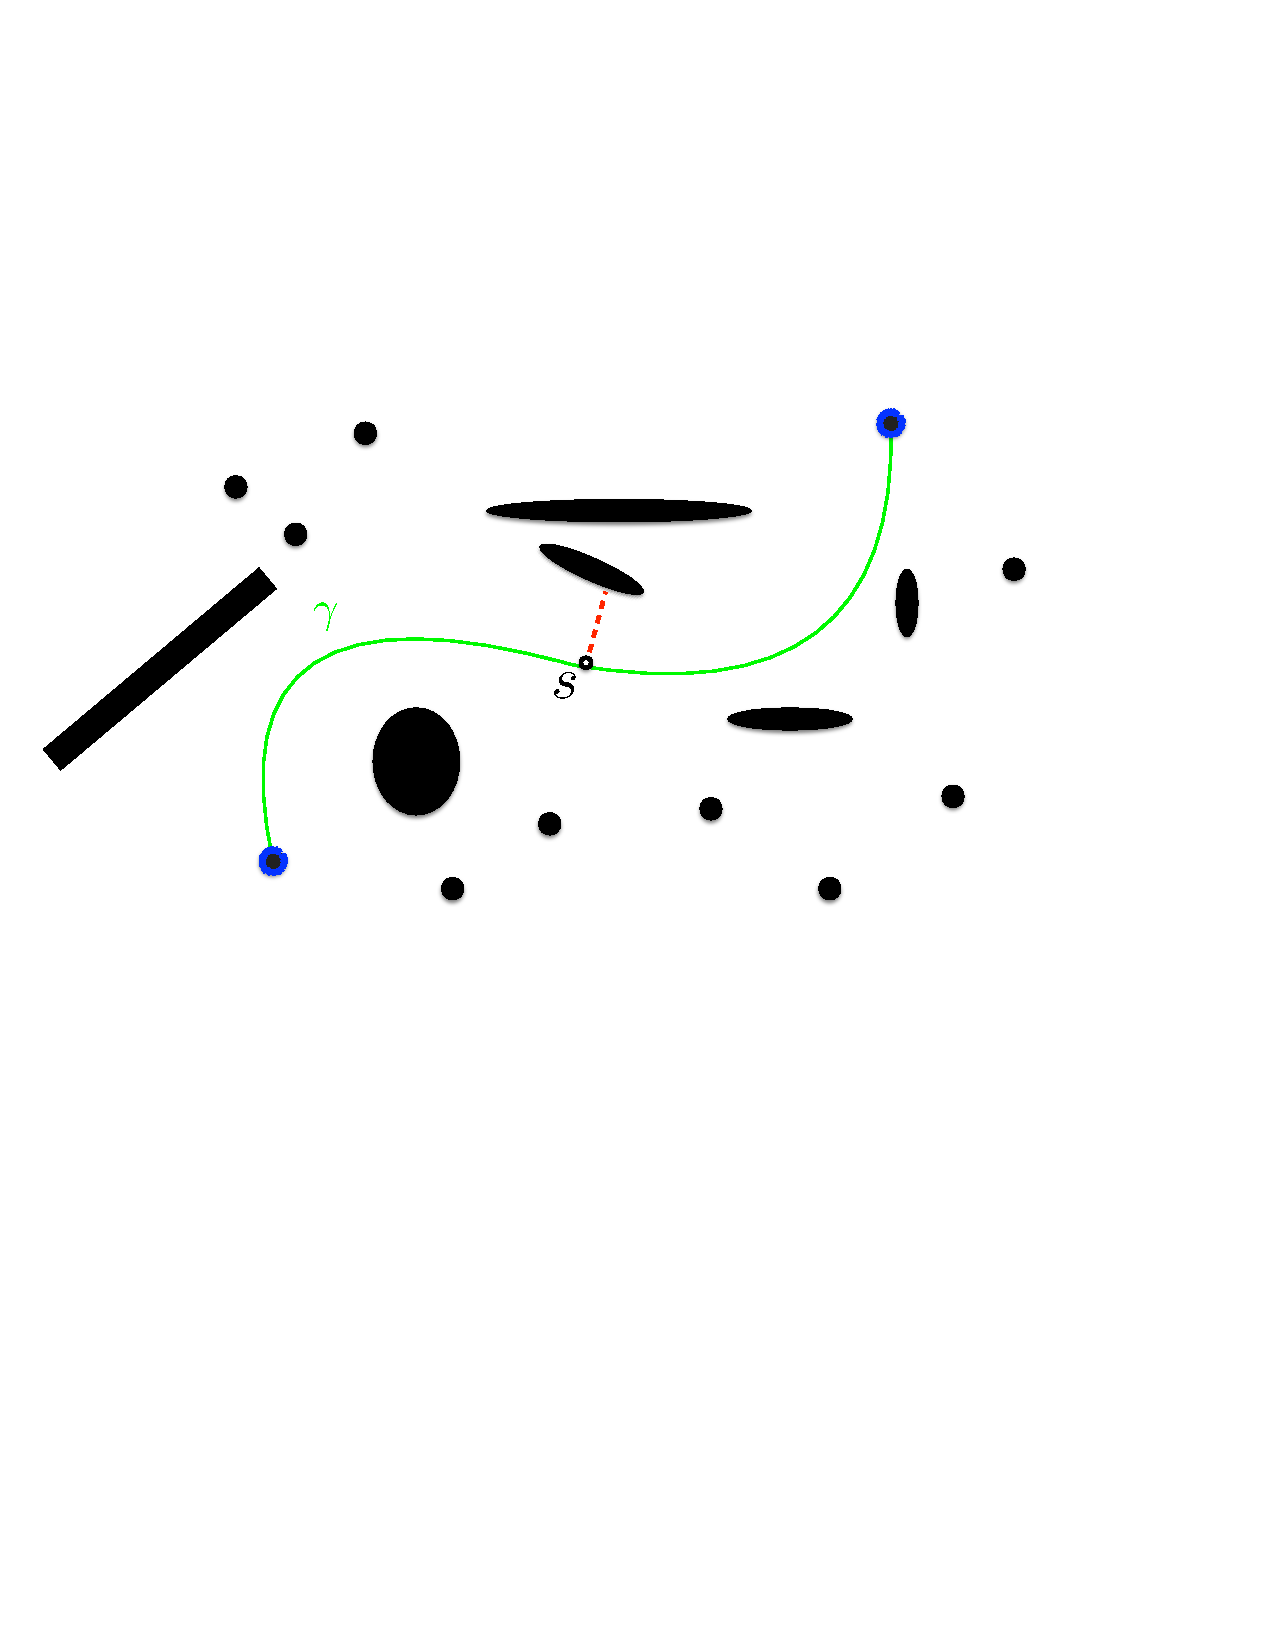
\includegraphics[width=0.3\textwidth]{Figures/example1.pdf}
    \caption{In this figure we have a collection of convex bodies in black.
      The length or cost of the green curve between the two blue points
      is the integral along the curve scaled by the distance to the nearest body.
    A curve may traverse a body at  no cost.}
  \label{fig:example}
\end{figure}



Conceptually, the density-based cost of a path is the weighted path length,
where each infinitesimal path piece is weighted with cost function $c$.
Density-based distances have been notable in the machine learning setting
for over a decade~\cite{}. To build a density-sensitive metric from density-based
distances, we would like a cost function $c$ that is small when close to
the data set, and large when far away. The Nearest Neighbor function is the
most natural candidate, and has been traditionally used as a proximity
measure between points and a data set in both the geometry and machine
learning settings~\cite{}. It has been used as such in Nearest Neighbor
(and $k$-NN) classification, $k$-means/medians/center clustering, finite
element methods, and any of the hundreds of methods that use Voronoi
diagrams or Delaunay triangulation as intermediate data structures.

\begin{definition} Given any finite set $P\subset \R^k$, there is a
real-valued function $\distto_P: \R^k\to \R$ defined as
$\distto_P(z) = 2\min_{x\in p} \|x-z\|$.  The \textbf{Nearest Neighbor Cost}
of a path $\gamma$ is $\len_{\distto_P}$, which we will shorthand to
$\len_N$.  
The \textbf{Nearest Neighbor Metric} between two points is
defined as $\dist_{\distto_P}$, which we short-hand as $\dist_N$.

The factor of $2$ in $\distto_P(z)$ is a
normalizing constant.
\end{definition}
The Nearest Neighbor metric, and density-based distances in general, are
examples of manifold geodesics (see~\cite{} for details). Manifold
geodesics are defined by embedding a point set into a continuous geometric
manifold, and computing the infimum length path on the manifold structure
between points.  Within computer science, dozens of foundational papers in
machine learning and surface reconstruction rely on manifold-based metrics
to perform clustering, classification, regression, surface reconstruction,
persistent homology, and more.  Manifold geodesics
predate computer science, and are the cornerstone of many fields of
physics and mathematics. Exactly computing geodesics is fundamental
to countless areas of physics including: the brachistochrone and
minimal-drag-bullet problem of Bernoulli and Newton, exactly determining a
particle's trajectory in classical physics (Hamilton's Principle of Least
Action), computing the path of light through a non-homogeneous medium
(Snell's law), finding the evolution of wave functions in quantum mechanics
over time (Feynman path integrals), and determining the path of light in
the presence of gravitational fields (General Relativity, Schwarzschild
metric). In mathematics, manifold geodesics appear in nearly every branch
of higher mathematics including differential equations, differential
geometry, Lie theory, calculus of variations, algebraic geometry, and
topology.  

One of the most significant problems on any manifold geodesic is how to
compute it exactly. Exact computation of manifold metrics is considered a
fundamental problem in mathematics and physics, dating back for four
centuries: entire fields of mathematics, including the celebrated calculus
of variations, have arisen to tackle this~\cite{}. Historically,
mathematicians placed strong emphasis on exact computation as opposed to
constant factor approximations. An algorithmic problem on manifold
geodesics, with modern origins, is to $(1+\eps)$ approximate these metrics
efficiently on a computer. The core difficulty in the first problem is that
geodesics are the minimum cost path out of an uncountable number of paths
that can travel 'anywhere' on the manifold structure. This makes exactly
computing these metrics challenging, even in the case of the Nearest
Neighbor metric for just four fixed points in two dimensions (the authors
are unaware of any easy method for this simplified task). 
The core tool for exactly
computing manifold metrics, calculus of variations, is intractable on the
nearest neighbor metric due to the metric's heavy dependence on the Voronoi
diagram of the point set, which can be quite complicated for even five
points in two dimensions (for more on this approach and its limitations,
see []). Calculus of variations can show that the optimal nearest neighbor
path is piecewise hyperbolic, but this is generally insufficient to exactly
compute the nearest neighbor metric - there are point sets where there are
many differentiable, piecewise hyperbolic paths between two data points with
different costs.


In this paper, we solve both problems: we exactly compute the Nearest
Neighbor metric in all cases, and we $(1+\eps)$ approximate it quickly.
Our approach is
based on conservative vector fields, contractive embeddings, Lipschitz
extensions, and minimum cost
flows on a graph. We combine these tools to prove that the nearest neighbor
metric is exactly equal to a shortest path distance on a geometric graph,
the so-called edge-squared metric, in all cases. This allows us to compute
the nearest-neighbor metric exactly for any given point set in polynomial
time, and it is the only known (non-trivial) density-based distance that can be computed
discretely.


\begin{definition} Given points in Euclidean space, the
\textbf{edge-squared graph} is the complete graph of Euclidean distances
squared. The \textbf{edge-squared metric} is half the shortest path distance
between two points on this graph. \end{definition}

Here, the factor of half in the definition is a normalizing constant.

\begin{theorem}\label{thm:NN} The nearest neighbor metric and edge squared
metric are equivalent for any compact point set in arbitrary dimension
\end{theorem}

The exact equality is realized when the nearest neighbor path is piecewise
linear, traveling straight from data point to data point. The edge squared
metric has been previously studied by multiple researchers in machine
learning and power-efficient wireless networks, but previously has only
been linked to the nearest neighbor metric by a fairly weak
3-approximation. Exact equality is considered highly surprising for at
least four reasons:

\begin{enumerate}

\item The optimal nearest neighbor path for two points not in the dataset
is generally piecewise hyperbolic. This holds true even when the
dataset is a single point, and was established by~\cite{}
using tools in Riemannian surfaces and the complex plane.
Meanwhile, Theorem~\ref{} implies an optimal nearest
neighbor path for two data points is piecewise linear!

\item There are simple and natural variants of the Nearest Neighbor metric,
for which no analog of Theorem~\ref{thm:NN} is known nor suspected.
These variants are known as the $q$-Nearest Neighbor
metric, for $1 < q < 2$, and we will formally define these
metrics later in the introduction. When $q=2$, these
metrics coincide with the Nearest Neighbor metric.
This
gives us a natural suite of metrics that smoothly converge
to the Nearest Neighbor metric, for which no theorem like
Theorem~\ref{thm:NN} is known.

\item Even for just three points in a right triangle configuration, there
exist an uncountable suite of optimal-cost paths between the two
endpoints of the hypotenuse. Each path in this uncountable
suite is piecewise hyperbolic, but, surprisingly, they all
have the exact same cost as the edge-squared distance. In
fact, the union of these paths is the entire right
triangle. Thus, lowering the Nearest Neighbor function
anywhere inside the triangle and using this to build a new
density-based distance will break
Theorem~\ref{thm:NN}. This establishes that the equality in
Theorem~\ref{thm:NN} is fairly tight.

\item This theorem holds for any compact point set, whether its $n$ points
in $n-1$ dimensional space or a countable union of compact geometric
objects in countably infinite dimension. The geometry of the latter can be
an extremely complicated object, and it is generally hard to prove
these types of results on arbitrary point sets.\gary{Hard sell this on a
union of line segments. Sounds surprising!}

\end{enumerate}

We can now tackle a second problem of interest for manifold geodesics,
which is efficiently $(1+\eps)$ approximating them. In this paper, we show
that the nearest neighbor metric admits $(1+\epsilon)$ spanners computable
in nearly-linear time, with linear size, for any point set in constant
dimension. Remarkably, these spanners are significantly sparser and faster
to compute than the theoretically optimal Euclidean spanners with the same
approximation constant, and nearly match the sparsity of the best known
Euclidean Steiner spanners. Moreover, if the point set comes from a
well-behaved probability distribution in constant dimension (a foundational
assumption in machine learning~\cite{}), we show that the nearest neighbor
metric has perfect $1$-spanners of nearly linear size. The latter result is
impossible for many non-density sensitive metrics, such as the Euclidean
metric. Both results rely on Theorem~\ref{thm:NN}, and significantly
improve the Nearest Neighbor spanners of Cohen et al in~\cite{}.

Theorem~\ref{thm:NN} and our spanner theorems solve two core problems of
interest for the nearest neighbor metric: exactly computing it for any
dimension, and approximating it quickly for both general point sets and
point sets arising from a well-behaved probability distribution in constant
dimension. This is the first work we know of that computes a manifold
metric exactly without calculus of variations, and we hope that our tools
can be useful for other metric computations and approximations. 

Besides for this contribution, we also generalize the Nearest Neighbor
Metric to the $q$-Nearest Neighbor metric (abbreviated $q$-NN for short),
and exactly compute this metric for all small point sets for all $q>2$. We
do this by equating it to the $q$-edge power metrics. Both the $q$-NN and
$q$-edge power metrics will be defined later.
\begin{theorem} \label{thm:qNN}
For point sets of up to $4$ points, the $q$-NN metric is exactly equal to
the $q$-edge power metric when $q>2$. This equality is false for all $q <
2, q\not=1$.
\end{theorem}
\begin{conjecture}\label{conj:qNN}
For any $n$ points, the $q$-NN metric is exactly equal to the $q$-edge
poewr metric when $q>2$.
\end{conjecture}

\tim{Move to contributions section?} We then use Theorem~\ref{thm:NN} to compute the persistent homology
of the Nearest Neighbor metric, a task important in computational geometry.
Additionally, we study the behavior of the Nearest Neighbor metric when the
points are drawn from a well-behaved distribution, as the number of points
goes to infinity. This turns out to converge w.h.p. to an extremely nice,
$1+o(1)$-approximation of a beautiful geodesic defined on the underlying
density previously studied by applied probability theorists. This
strengthens the work of Hwang, Hero, and Damelin, who showed that the
Nearest Neighbor metric converged to a $O(1)$-approximation of this
beautiful geodesic. This geodesic is a beautiful and natural generalization
of both Euclidean distances and a distance fundamental for clustering using
level-set methods. We further show that $q$-edge power metrics (and thus,
it is hoped, the $q$-Nearest Neighbor metrics) are natural generalizations
of maximum-edge-length distances on Euclidean MSTs, which in turn are
fundamental for celebrated clustering methods like single-linkage
clustering~\cite{}. This implies that the $q$-edge power metric, and the
Nearest Neighbor metric, can be used to generalize popular methods in
clustering.

Our final set of theorems regards the $q$-screw simplex, the core geometric
object in our proof of Theorem~\ref{thm:NN} and its generalizations. The
$q$-screw simplex was first discovered by John Von Neumann and Issai
Schoenberg. It is defined by taking $n$ points anywhere on a line, taking
the $1/q$ power of the distances, and isometrically embedding the resulting
distances into Euclidean space. The fact that such an embedding exists was
the core contribution of Schoenberg and Von Neumann in~\ref{}. The central
role of $q$-screw simplices in our proofs motivates us to develop new
theorems on the geometry of these objects. Surprisingly, we find that these
simplices are useful for proving generalizations of Von Neumann's work, and
are deeply related to spectral graph theory.

Isometric embedding is a topic of wide interest in the field of metric
geometry, and has been studied for many decades. Von Neumann and Issai
Schoenberg proved in their seminal work that any $q$-screw simplex is
isometrically embeddable in $l_2$. We extend their work to prove a stronger
result: 
\begin{theorem}
Any $q$-screw simplex isometrically embeds into the space of
Effective Resistance metrics, for all $q>1$.
\end{theorem}
Simple metrics like the square in $l_2$ are
not isometrically embeddable into this class of metrics, and thus, most
Euclidean metrics are not expected to isometrically embed into Effective
Resistance distance. Isometric embedding into effective resistance metrics
has been a popular question in spectral graph theory ~\cite{}, and this is
the first result we know of where a geometric distance defined without an
obvious underlying electrical network embeds isometrically into Effective
Resistances. We prove this isometry by showing a deep link between
$q$-screw simplices and a differential operator known as the fractional
Laplacian, which has wide applications in fields including fractional
quantum physics~\cite{}, cell membrane biology~\cite{}, financial
mathematics~\cite{}, Brownian motion~\cite{}, differential
equations~\cite{}, semi-groups~\cite{}, Fourier analysis~\cite{}, and
more~\cite{}. This further allows us to show that fundamental geometric
quantities like circumcenters (essential for Voronoi diagram construction)
and volumes on the $q$-screw simplex can be determined using fundamental
primitives on graph Laplacians, in this case Laplacian system solving and
Laplacian determinant estimation respectively. The fractional Laplacian can
be interpreted as a natural example of a geometric resistive graph, first
introduced by Alman et. al. in ~\cite{}. We further conjecture that taking
the $q^{th}$ root of any tree metric is isometrically embeddable into
effective resistance, which would imply that the Gomory Hu tree (and thus
the inverse min-cut distance) embeds isometrically into effective
resistances.

We also provide the first known closed form finite-dimensional embedding of
the $q$-screw simplex into Euclidean space, when $q>2$. The work of Von
Neumann et. Al. proved the simplex's existence for $q>1$ by embedding it
into infinite dimensional Hilbert space using theorems from complex
analysis, functional analysis, infinite dimensional Hilbert space theory,
and Fourier analysis. Our embedding uses only elementary techniques of
eigenvector computation on finite matrices. We hope that this embedding
makes the work of Von Neumann and Schoenberg more accessible. We use our
new embedding to state and prove a generalization of Von Neumann and
Schoenberg’s theorem (on the embeddability of the $q$-screw simplex):

\begin{theorem}~\label{thm:l1} For points $p_1, \ldots p_n \in
\mathbb{R}^n$ and any $q > 1$, the metric $D(p_i, p_j) = |p_i-p_j|_1^{1/q}$
is isometrically embeddable into $l_1$.\end{theorem}
This mirrors
Schoenberg's famous theorem that any finite $l_2$ metric, raised to the
$1/q$ power for $q > 1$, is isometrically embeddable in $l_2$.

  \section{Our Results}
Our primary results are Theorems~\ref{thm:NN} and~\ref{thm:qNN} on the
computing the Nearest Neighbor and $q$-Nearest Neighbor metrics
respectively, which rely
on fairly intricate and novel mathematical proof techniques. Both of these
use a minimum cost flow generated from a conservative vector field to keep
track of the $q$-NN path length, and rely on the geometry of a special
simplex called the
$q$-screw simplex. Our proof techniques, theoretically, can prove
approximations between metrics as well as exact equalities, and may be
uesful for other more general metrics based on data points. This is the
first result we know of whose proof combines
conservative vector fields, simplex geometry, Lipschitz extensions in
geometry, and minimum cost flows on a graph. It is also the first result we
know of that eschews calculus of variations for exact manifold metric
computation.

These results form the core mathemtaical contribution of our paper.

\subsection{Other Contributions}
Besides for these contributions, we also tackle a range of problems
significant for any metric on a data set.  Some of the most important
problems on any metric are: how to $(1+\eps)$ approximate them efficiently
using sparse data structures, and how the metric behaves in the limit as
the point set is a large number of points drawn from a probability
distribution. The former is important to compute the metrics in practice.
The latter is important since it is highly desirable that
this limit converge to a metric that has desirable properties, or else
clustering with such a metric may generate non-intelligible results for
large datasets.  Persistent homology of metrics space is also a central
tool in topological data analysis, among other fields~\cite{}, and many
papers have devoted themselves to computing such homologies ofr a wide
variety of metrics. Finally, it is important to relate metrics
like the Nearest Neighbor metric to famous, well-established metrics like
$l_2$, inverse min-cut distance, or
the maximum edge length among a path in an MST.
We will show that the
Nearest Neighbor metric is in fact one of a suite of simple metrics (the
$q$-edge power metrics) which naturally generalize both maximum-edge MST
distance and Euclidean distance, the latter of which covers inverse min-cut
idstances via the Gomory Hu tree.  This helps put our metrics in a broader
and more interpretable context, and ensures that clustering with these
$q$-power metrics is a generalization of more traditional clustering
techniques including $k$-means, $k$-centers, and level set methods.

In this paper, we present significant progress all of these problems. Our
spanner and convergence results hold assuming constan dimension, and our
persistent homology results and our relation to more famous metrics hold for
$n$ points in any dimension. While the proofs of these results range from
the standard to the intricate, we hope that the sheer number of results
that can be stated (as well as their quality) inspires future researchers
to further study density-based distances and their related geometric objects.

Our spanner theorems are as follows:

 %% \begin{theorem} \label{thm:NN} Given a point set $P \in \mathbb{R}^d$, the edge-squared metric on $P$
%%   and the Nearest Neighbor Metric on $P$ are always equivalent.
%% \end{theorem}

\begin{theorem} \label{thm:general-spanner}
  For any set of points in $\mathbb{R}^d$ for constant $d$, there exists a $(1+\eps)$
  spanner of the Nearest Neighbor Metric
  with size $O\left(n\eps^{-d/2} \right)$ computable in time
  $O\left(n \log n + n\eps^{-d/2}\log{\frac{1}{\eps}}\right)$. The
  $\log{\frac{1}{\eps}}$ term goes away given access to an algorithm
computing floor function
in $O(1)$ time.
\end{theorem}

\begin{theorem} \label{thm:distribution-spanner}
Suppose points $P$ in Euclidean space are drawn i.i.d from a Lipschitz probability density bounded
above and below by a constant, with support on a
smooth, connected, compact manifold with intrinsic dimension $d$,
  and smooth
  boundary of bounded curvature. Then w.h.p. the $k$-NN graph of
  $P$ for $k = O(2^d \ln n)$ and edges weighted with Euclidean
  distance squared, is a $1$-spanner of the Nearest Neighbor
  metric on $P$.
\end{theorem}


Theorem~\ref{thm:ditsribution-spanner} tackles a common setting in machine
learning, where points are assumed to be from a well-behaved ditsribution.
These assumption is foundational to the field of machine learning.
Although the restrictions on the distribution seem fairly limiting (and
naively, do not even cover the case of a simple Gaussian), they turn out to
be far more flexible than they seem, and are common in the machine learning
literature. They can be modified to gain information on most relevant
distributions (for example, they cover the
case of a Gaussian where the thin tail is removed, which turns out to
contain most of the information of a Gaussian).
Theorem~\ref{thm:general-spanner} generalizes the results of Cohen et. al.
in~\cite{cohen15approximating}, who showed nearly linear size spanners in
nearly linear time, but with significantly worse $\eps$ dependence. Note
that these spanners can be computed even faster than the optimal known
Euclidean spanner, indicating that density-sensitive metrics like the
Nearest Neighbor metric may have interesting algorithmic possibilities that
standard distances like $l_2$ and $l_1$ don't have.

Results on the geodesics, etc. will be presented in their appropriate
section.

\subsection{Properties of the $q$-screw simplex, and related results}
Our secondary results are Theorems~\ref{thm:ER} and~\ref{thm:l1}, which are
isometric embeding results that emerge from studying the geometry of the
$q$-screw simplex.  These results are of independent interest from the main
text on density-sensitive distances, but are linked since the $q$-screw
simplex is the fundamental geometric object in our proofs of
Theorem~\ref{thm:NN} and~\ref{thm:qNN}.
Theorem~\ref{thm:ER} is one of the few results on isometrically embedding a
geometric simplex into effective resistance, where the underlying
electrical network is not apparent. It also establishes links between
$q$-screw simplices and the considerably large field of spectral graph theory,
which we hope sets the stage for fertile future work.
Theorem~\ref{thm:l1} generalizes the $q$-screw simplex embeddability result
of Schoenbreg and Von Neumann, and mirrors a famous theorem of Schoenberg.
To the author's knowledge, this theorem was not known or even guessed
before.

  \section{Outline}
%   Definitions of the nearest neighbor metric distance, and of the
%     edge-squared metric, are provided in
%    Section~\ref{sec:definitions}.
%
Section~\ref{sec:NN} contains the proof of Theorem~\ref{thm:NN},
equating the edge-squared metric and nearest neighbor metric distance in
all cases. It should be noted that our proof is robust enough to handle not
just finite point sets, but also countably infinite collections of disjoint
path-connected, compact sets. Remarkably, there is no restriction on the convexity or
simply-connectedness of these sets.

As an example of using the nearest neighbor metric to compute intrinsic structure, Section~\ref{sec:persistence} shows how Theorem~\ref{thm:NN} allows us to compute the persistent homology of the nearest neighbor metric.
Section~\ref{sec:general-spanner} outlines a proof of Theorem~\ref{thm:general-spanner}, and compares our spanner to new lower
bounds
on the sparsity of $(1+\eps)$-spanners of the Euclidean metric.
We outline a proof of Theorem~\ref{thm:distribution-spanner} in
Section~\ref{sec:distribution-spanner} and discuss its implications.

Section~\ref{sec:edge-power} introduces the $p$-power metrics. We show
that Euclidean spanners and Euclidean MSTs are special cases of
$p$-power spanners. We show how
clustering algorithms including $k$-means, level-set methods,
and single linkage clustering, are special cases of
clustering with $p$-power metrics. $p$-power metrics are identical to the
Neighbor metric when $p=2$.


Conclusions and open questions are in
Section~\ref{sec:conclusions}. Full proofs for
Theorems~\ref{thm:distribution-spanner},~\ref{thm:general-spanner}
are contained in the Appendix.

  
\begin{lemma}\label{lem:flow} There exists a function $\Conv$ such that for
any
path piece $\phi$ running from $x$ and $x+\Delta(x)$, $\len_{qN}(\phi) \geq
MCF_{G'}(B'(x+\Delta(x))-B'(x))$. Here, $MCF_{G'}(d)$ for $d \in
\mathbb{R}^{2^n}$ represents the minimum cost flow on $G'$ satisfying demands
$d$ on the vertices of $G'$.

\end{lemma}

\begin{lemma}\label{lem:radius} Let $S = s_1 < s_2 < \ldots s_{|S|}$, and $T =
t_1 < \ldots \leq t_{|T|}$, where $S, T \subset \{0,1,\ldots n-1\}$ and $S$ and
$T$ differ by exactly one element. Let $R_S$ denote the circumradius of the
$q$-screw simplex formed by $s_1, s_2, \ldots s_n$. ~\tim{Define what
'being formed by' means.} If

\begin{align}\label{eq:radius} |(R_{S})^q-(R_{T})^q| \geq
|(s_{|S|}-s_1)/2^q-(t_{|T|}-t_1)/2^q|, \end{align}

then the shortest path in $G'$ equals the shortest path in $G$.

\end{lemma}

Note that this inequality is always an exact equality for $q=2$. The proof of
this lemma is combinatorial:

\begin{proof}

\end{proof}

Therefore, if Equation~\ref{eq:radius} holds for any set of $k$ points, and
Lemma~\ref{lem:flow} and~\ref{lem:radius} are proven, then we've proven
Theorem~\ref{thm:general} for any $k$ element point set.

\textbf{Proof of Lemma~\ref{lem:flow}}

\textbf{Proof of Lemma~\ref{lem:radius}}

\begin{lemma} $SP_{G'}(v_0, v_n) \leq SP_G(x_0, x_n)$

\end{lemma}

\begin{proof}

The distance from $v_0$ to $v_{\{0,n-1\}}$ on the graph is equal to
$u_{n-1}-u_0$ (NORMALIZE THINGS PROPERLY, INDEX THINGS PROPER, SET COMMON
VARIABLE NAMES), and the distance from $v_{\{0, n-1\}}$ to $v_{n-1}$ is the
same. Thus, this path from $v_0$ to $v_n$ equals $SP_G(x_0, x_n)$, as the
latter is trivially equal to $u_{n-1} - u_0$.

\end{proof}

Thus, it suffices to prove that

\[ SP_{G'}(v_0, v_n) \geq SP_G(x_0, x_n) \]

%%%% GAP

\subsection{Construction of $\Conv$}

In this section, we prove we Lemma~\ref{lem:flow}. We construct a function
$\Conv:\mathbb{R}^n \rightarrow \mathbb{R}^{2^n}$ assigning every point in
Euclidean space to a vector, representing a convex combination of vertices
in $G'$. We will build $\Conv$ separately for each Voronoi cell, and show
it is piecewise continuous across boundaries of Voronoi cells. 
However, to simplify our arguments, we further divide up each Voronoi cell
into simplices similar to the dissection in a barycentric subdivision.
However, rather than barycenters, we use circumcenters, so we are
more-precisely dividing up the $q$-screw simplex with a circumcentric
subdivision. \tim{define circumcentric/barycentric subdivision}

Let $p_{S}$ be the circumcenter of points $\{p_s | s \in S\}$ when $S
\subset \{1, 2, \ldots n\}$. A simplicial cell in the circumcentric subdivision is
defined by a permutation $a_0, a_1, \ldots a_{n-1}$ of $\{0, 1, \ldots
n-1\}$ as follows: let
$A_i = \{a_0, a_1, \ldots a_{i}\}$. Then the vertices $\{p_{A_i} | 0 \leq i
< n\}$ are the vertices of the simplicial cell.  \tim{Move this definition
upwards somewhere?} Each Voronoi cell is the disjoint~\tim{not exactly
disjoint} union of some of
these cells, and the cells partition the simplex \tim{This isn't quite
true: its only true for special geometry cells, but we don't particularly
care... how can I make this point clear?}. Our general strategy is to
create $\Conv$ on each simplicial cell, and show that is piecewise
continuous across the boundaries of simplicial cells.

To simplify our notation, we define $\pr_i$ to be $p_{A_i}$. \tim{Make sure
all points are $p$, not $x$. $\xr_k$ is later used to coordinate-wise split
up $x$}.

%Define $\pr, \xr, \Rr, \Convr$ here. Points $\pr$ numbered from $0$ to $k-1$.
%Here, $\xr$ is numbered $1$ through $k-1$. $B$ is $0$ through $k-1$
%indexed.


By the construction of circumcentric subdivisions, 
the line $\pr_{i}\pr_{i+1}$ is perpendicular to
$\pr_{i+1}\pr_{i+2}$ for all $i$. These lines define a natural
orthonormal coordinate axis. Thus,
for any $\xr$ in the convex hull of $\pr_i$, we can write $\xr$ in
coordinates $(\xr_0, \xr_1, \ldots \xr_{n-2})$, where the $i^{th}$ coordinate
axis is parallel to $\pr_i \pr_{i+1}$.

Next, we introduce how $\Convr$ is defined on the vertices $\pr_{i}$. Here,
$\Convr_i$ is shorthand for the value of $\Convr$ on $\pr_{i}$.

\begin{align}
\Convr(\xr)_i = \frac{
\left(\sum_{s=0}^{i-1} {\xr_s}^2\right)^{q/2} -\left(\sum_{s=0}^{i-2}
{\xr_s}^2\right)^{q/2}
}
{
\Rr_i^q - \Rr_{i-1}^q
} - \sum_{i < j < n} \Convr(\xr)_j
\end{align}

for all $1 \leq i \leq n-1$, and \tim{make sure you replace all k's with
n's, and claim that you're dealing with simplices of full dimension. You
may want to say that the proof is counterintuitive since simplices of full
dimension are usually considered harder?}

\[ \Convr(\xr)_0 = 1 - \sum_{0 < j < n} \Convr(\xr)_j
\]

The key feature about $\Convr$ is that

\[\sum_{j=i}^n \Convr(\xr)_j= \frac{
\left(\sum_{s=0}^{i-1} {\xr_s}^2\right)^{q/2} -\left(\sum_{s=0}^{i-2}
{\xr_s}^2\right)^{q/2}
}
{
\Rr_i^q - \Rr_{i-1}^q
}\]

for all $i > 0$, and for $i = 0$ the LHS evaluates to $1$.

Since we defined this function piecewise, we need to check that this
function is piecewise continuous.

\begin{lemma} If $\xr$ is on a face of $\pr_0, \ldots \pr_n$, then
$\Convr(\xr)$ has non-zero coordinates only on that face. Furthermore, the
coordinates depend only on SOMETHING.

\end{lemma}

\begin{proof}

\end{proof}

Now we are ready to prove our core lemma:

\begin{lemma} For $x$ and $x+\Delta(x)$ in the convex hull of $\pr_1,
\ldots \pr_k$, the distance:

\[ \|x-\pr_1\|^{q-1} \cdot \|\Delta(x)\| \geq
F\left(\Convr(x+\Delta(x))-\Convr(x)\right)\]

where $F(d)$ is the unique cost of a flow satisfying demand $d \in
\mathbb{R}^n$ on $\Gr$.

\end{lemma}

Here, the left hand side represents the $q$-NN cost of a path piece from
$x$ to $x+\Delta(x)$, and the right hand side is the unique cost of the
induced flow on graph $G'$, with the restriction that the flow is only
nonzero on the vertices $\pr_i\pr_{i+1}$ for any $0 \leq i < n$. This flow
is unique since we forced our flow to be non-zero only on the edges
$\pr_i\pr_{i+1}$, which form a line graph; and for any set of demands on
vertices of a line, there is a unique flow satisfying those demands.

\begin{proof} For any edge $\pr_i\pr_{i+1}$, the cost of a flow (satisfying
some set of demands whose sum is $0$) on that edge is the absolute value of
the sum of the demands on vertices $\pr_{i+1} \pr_{i+2}, \ldots \pr_n$,
multiplied by the cost of the edge from $\pr_i$ to $\pr_{i+1}$. This
quantity comes out to be:

\begin{align} &\left(\Rr_{i+1}^q-\Rr_{i}^q \right) \sum_{j=i+1}^n \Convr(\xr)_j
\\
\label{eq:flow-cost}
&=\left(\sum_{s=0}^{i-1} {\xr_s}^2\right)^{q/2} -\left(\sum_{s=0}^{i-2}
{\xr_s}^2\right)^{q/2}.
\end{align}

As $\Delta(x)$ goes to $0$, the change in Expression~\ref{eq:flow-cost} is

\begin{align}
\begin{split}
\label{eq:flow-cost-on-edge}
&
\left(q\xr_0 \left(\sum_{s=0}^{i-1} \xr_s^2 \right)^{q/2-1} -
q\xr_0\left(\sum_{s=0}^{i-2} \xr_s^2 \right)^{q/2-1} \right) \Delta(\xr)_0
\\
&+
\left(q\xr_1 \left(\sum_{s=0}^{i-1} \xr_s^2 \right)^{q/2-1} -
q\xr_1\left(\sum_{s=0}^{i-2}\xr_s^2 \right)^{q/2-1} \right) \Delta(\xr)_1
\\
&+ \ldots
\\
&+
\left(q\xr_{i-2} \left(\sum_{s=0}^{i-1} \xr_s^2 \right)^{q/2-1} -
q\xr_{i-2}\left(\sum_{s=0}^{i-2}\xr_s^2 \right)^{q/2-1}
\right)\Delta(\xr)_{i-2}
\\
&+
\left(q\xr_{i-1} \left(\sum_{s=0}^{i-1} \xr_s^2
\right)^{q/2-1}\right)\Delta(\xr)_{i-1},
\end{split}
\end{align}
Since 
\[
q\xr_j\left(\sum_{s=0}^{i-1} \xr_s^2\right)^{q/2-1} - q\xr_j\left(\sum_{s=0}^{i-2}
\xr_s^2 \right)^{q/2-1}\]
is always non-negative (only when $q \leq 2$), we get that the absolute value of
Expression~\ref{eq:flow-cost-on-edge} is bounded above by:
\begin{align}
\begin{split}
\label{eq:flow-cost-upper-bound}
&
\left(q\xr_0 \left(\sum_{s=0}^{i-1} \xr_s^2 \right)^{q/2-1} -
q\xr_0\left(\sum_{s=0}^{i-2} \xr_s^2 \right)^{q/2-1} \right)
|\Delta(\xr)_0|
\\
&+
\left(q\xr_1 \left(\sum_{s=0}^{i-1} \xr_s^2 \right)^{q/2-1} -
q\xr_1\left(\sum_{s=0}^{i-2}\xr_s^2 \right)^{q/2-1} \right) |\Delta(\xr)_1|
\\
&+ \ldots
\\
&+
\left(q\xr_{i-2} \left(\sum_{s=0}^{i-1} \xr_s^2 \right)^{q/2-1} -
q\xr_{i-2}\left(\sum_{s=0}^{i-2}\xr_s^2 \right)^{q/2-1}
\right)|\Delta(\xr)_{i-2}|
\\
&+
\left(q\xr_{i-1} \left(\sum_{s=0}^{i-1} \xr_s^2
\right)^{q/2-1}\right)|\Delta(\xr)_{i-1}|,
\end{split}
\end{align}

Expression~\ref{eq:flow-cost-upper-bound} is an upper bound on the cost of
a flow along edge $\vr_i\vr_{i+1}$\tim{Is this the right indexing for
edges?} induced by a path from $x$ to $x+\Delta(x)$. Now we sum this across all $i$ to get an overall cost upper bound, and group by
$\Delta(\xr)_i$ for fixed i. The sum telescopes beautifully, and we get:
\begin{align}
&\left(q\xr_0\left(\sum_{s=0}^{n-2} \xr_s^2\right)^{q/2-1}\right)| \Delta(\xr)_0|
\\&+
\left(q\xr_1\left(\sum_{s=0}^{n-2} \xr_s^2\right)^{q/2-1}\right)| \Delta(\xr)_1|
\ldots
\\& +
\left(q\xr_{n-1}\left(\sum_{s=0}^{n-2} \xr_s^2\right)^{q/2-1}\right)| \Delta(\xr)_{n-2}|
\end{align}
This expression, by Cauchy Schwarz, is upper bounded by
\[
\sqrt{\sum_{s=0}^{n-2} \Delta(\xr)_s^2} \cdot \left(q\sqrt{\sum_{s=0}^{n-2}
\xr_s^{q-1}}\right)
\]
Which is exactly the $q$-NN distance.

\end{proof}

Note that this function is piecewise continuous on the boundary. Therefore,
we have shown that the $q$-NN cost of any path piece is less than the
min-cost flow on $G’$ satisfying
$\Conv\left(x+\Delta(x)\right)-\Conv\left(x\right)$ for infinitesimal
$\Delta(x)$, as desired.

So far, the only property our flow construction used is that the points
$x_0, x_1, \ldots x_n$ have Voronoi subdivisions defined by $\pr_{a_0}$,
$\pr_{a_0a_1}$, \ldots $\pr_{a_0a_1\ldots a_k}$, for some $a_0, ldots a_k
\subset \{0, 1, \ldots n\}$. (DOES THIS WORK FOR ANY GEOMETRY, OR DO I NEED
THE INTERIOR CIRCUMCENTER PROPERTY?).

Thus, we have proven a core lemma:

\begin{lemma}\label{lem:qNN-GPrime}

The $q$-NN distance between two points in a point set is lower bounded by
the shortest path between the two corresponding points in $G’$. Here, $G’$
is constructed as in Definition~\ref{def:GPrime}

\end{lemma}

We now prove the following two lemmas, completing our proof of
Theorem~\ref{thm:NN} and Theorem~\ref{thm:qNN} respectively.

\begin{lemma}\label{lem:edge-squared-GPrime} Let $G$ be the edge-squared graph
(DEFINE), and let $G’$ be defined as in Definition~\ref{def:GPrime} for $q=2$.
The shortest path in $G’$ is the same as the shortest path in $G$, when the
initial point set generating $G$ and $G’$ is a $2$-screw simplex.

\end{lemma}

\begin{lemma}\label{lem:q-edge-power-GPrime} Let $q > 2$. Let $G$ be the
$q$-edge power graph, and $G’$ be defined as in Definition~\ref{def:GPrime}
(MAKE SURE THE DEFINITION IS Q DEPENDENT). The shortest path in $G’$ is the
same as the shortest path in $G$, when the initial point set generating $G$
and $G’$ is a $q$-screw simplex with $4$ points.

\end{lemma}

Combined with Theorem~\ref{thm:screw-simplex-reduction},
Lemmas~\ref{edge-squared-GPrime} and~\ref{q-edge-power-GPrime} prove
Theorems~\ref{thm:NN} and~\ref{thm:qNN} respectively. Moreover, we make the
following conjecture, which we have some computational evidence for (See
Appendix~\ref{} for details):

\begin{conjecture}\label{conj:qNN}

For $q>2$, let $G$ and $G’$ be defined as in
Lemma~\ref{lem:q-edge-power-GPrime}. Then the shortest path in $G’$ is the same
as the shortest path in $G$.

\end{conjecture}

If this were true, it would prove that the $q$-edge power metric and the
$q$-NN metric were equal for all $q>2$.


Now, our proof will proceed in two parts. First, we construct a function
$B':\mathbb{R}^n \rightarrow \mathbb{R}^{2^n}$ assigning every point in
Euclidean space to a vector, representing a convex combination of vertices in
$G'$. We build $B'$ such that $B'(v_S)= e_S$, where $e_S$ is the unit vector
with $1$ in the dimension indexed by $S$. Next, we lower bound the
Nearest-Neighbor cost of an infinitesimal path piece. If the infinitesimal path
piece runs from $x \in \mathbb{R}^n$ to $x+\Delta(x)$, where both $x$ and
$x+\Delta(x)$ are in the same circumcentric subdivision (DEFINE), then we lower
bound it with some flow on the graph $G'$ satisfying demands $B'(x+\Delta(x)) -
B'(x)$.

If we can find a cost function $B'$ with these properties, we can integrate
over all the infinitesimal path pieces to show that the $p$-NN cost of a path
from $x_0$ to $x_{n-1}$ is lower bounded by some flow on $G'$. This is a unit
flow from $x_0$ to $x_n$. If we furthermore have that the shortest path on $G'$
equals the shortest path on $G$, then we have:

$$NN(path) \geq Q' \geq SP_{G'}(v_0, v_n) = SP_{G}(x_0, x_n).$$

Here, $Q'$ represents the cost of some flow from $v_0$ to $v_n$ on $G'$. Here,
$SP_{G'}(v_0, v_n)$ is the shortest path from $v_0$ to $v_n$ on $G'$ and
$SP_G(x_0, x_n)$ is the shortest path from $x_0$ to $x_n$ on the q-edge power
graph of the $q$-screw simplex.

Our proof then consists of two parts: the first is finding a graph $G'$ and
showing $SP_{G'}(v_0, v_n) = SP_G(x_0, x_n)$ (STANDARDIZE INDICES). The second
is finding a function $B'$ satisfying our desired properties listed in our
strategy. In the remainder of this section, we build our graph $G'$ and
establish

a discrete, sufficient-but-not-necessary criterion for when $SP_{G'}(v_0, v_n)
= SP_G(x_0, x_n)$. Then we build a function $B'$ and prove that $NN(path) \geq
Q'$, where the path runs from $v_0$ to $v_1$.

We then show that this necessary-but-not-sufficient criterion holds for any $5$
point $q$-screw simplex, thereby showing that the $q$-edge power metric equals
the $q$-NN metric for all $5$ point sets. We further conjecture that this
criterion holds for any $n$ points, but the authors are currently unable to
prove it.

Therefore, we have provided a sufficient but not necessary criterion for which
the $q$-edge power metric equals the $q$-NN Metric on the $q$-screw simplex.
Furthermore

Then we establish a discrete criterion in which $G' \geq G$. We then prove this
criterion holds for all sets of $5$ points in arbitrary dimension, and
conjecture that it holds for all sets of $n$ points in arbitrary dimension.


\section{Fractional Laplacian}

In this section, we prove that the $q$-screw simplex distances arise as
effective resistance of the Fractional Laplacian, for powers $s = -1/2-1/q  $,
when $q > 2$. 

Preliminaries: Fractional Laplacian. 

We present two definitions: the first definition is based on taking the limit
of graph Laplacians raised to the fractional power (which are known in folklore
to be graph Laplacians themselves), and the second definition is based on
taking fractional powers of the Laplacian differential operator when the latter
is written in terms of its Eigenvectors, the Fourier bases.

In this work, we build on Von Neumann and Schoenberg’s proof of embeddability
of the $q$-screw simplex. Their work (slightly simplified by the authors of
this paper) shows that the $q$-screw simplex for $q > 1$ can be embedded in
infinite dimensional Hilbert space, by the embedding $f: mathbb{R} \rightarrow
L_2$ defined as:

\begin{align}\label{eq:screw-embedding} f(x) = \frac{e^{i\omega
x}}{\omega^{1/2+1/q}} \end{align} Where $f(x)$ is a function in the variable
$\omega$.

The proof of their embedding hinges on the following remarkable integral
formula: \[ \| x_1 – x_2 \|_2^{1/q} = \frac{sin^2(\omega(x_1-x_2)
)}{\omega^{1+2/q}},  \] the left hand side of which is the norm for
Equation~\ref{eq:screw-embedding}. This integral formula is a classical
integral formula~\cite{}, and can be proven using Jordan’s integration theorem
from complex analysis~\cite{,}.

Notice that the step function $S_x$, which is $1$ between $-x$ and $x$ and $0$
elsewhere, can be written in Fourier bases as: \begin{align} \label{eq:step}
S(x) = frac{e^{i\omega x}}{\omega}.  \end{align} Equation~\ref{eq:step} is a
classic result, dating back to the earliest days of functional analysis.
However, this formulation compared with Equation~\ref{eq:screw-embedding}
practically invites us to use the Fractional Laplacian, when viewed through the
Eigenvector lens in Section~\ref{sec:frac-lap-eigenvector}.

Therefore, we can write Equation~\ref{eq:screw-embedding} as: \[ f(x) =
\Delta^{1/4-1/(2q))} Step = \Delta^{1/4-1/(2q)} (\Delta^{-1/2} \delta_{-x} -
\delta_{x}) = \Delta^{-1/4-1/(2q)} (\delta_{-x} - \delta_{x}) \] In the above
expression, $\delta_x$ represents the Dirac Delta function. DEFINE $\Delta$ in
this case!!!! Here, the second part of the equation is a standard manipulation
in differential equations, as $\Delta^{1/2}$ is conceptually similar to the
integral operator. For more on manipulations with this fractional Laplacian
operator, see~\ref{}.

And thus $|x-y|^{2/q} = ||f(x)||_2^2$ can be written as: \begin{align}
(\delta_{-x} - \delta_{x})^T \cdot \Delta^{-1/2-1/q} \cdot (-\delta_{-x} –
\delta_{x}) \end{align} Which is an effective resistance distance. This can be
seen since $\Delta^{-1/2-1/q}$ can be written as the limit of fractional graph
Laplacians (which are in turn graph Laplacians, by Lemma~\ref{}). Given a
finite screw simplex, our distance is thus the limit of the Schur complement of
these graph Laplacians onto a finite point set, which is the limit of a
sequence of graph Laplacians. It can be seen easily that such graph Laplacians
must converge, and the limit of this convergence is a graph Laplacian whose
effective resistance distance are the screw simplex distances. This proves
Theorem~\ref{thm:embed}. 

   % % !TeX root = main.tex

\subsection{Definitions and Preliminaries} % (fold)
\label{sec:definitions}

\noindent \textbf{Edge-squared metric:}  For $x\in \R^d$, let $\|x\|$ denote the Euclidean norm.
  For a set of points $P\subset \R^d$:

  \begin{definition}
  The edge-squared metric for $a,b\in P$ is
  \[
    \dist_2(a,b) = \min_{(p_0,\ldots, p_k)}\sum_{i=1}^k \|p_i - p_{i-1}\|^2,
  \]
  where the minimum is over sequences of points $p_0,\ldots, p_k\in P$ with $p_0 = a$ and $p_k = b$.
  \end{definition}
%  \tim{Anything on wireless networks here? Or other prelims?}

\vspace{3 mm}
\noindent \textbf{Nearest-neighbor geodesic distance:}
  Another metric on the points of $P$ is called the nearest-neighbor
  geodesic distance, and is denoted $\dist_N$.
This distance was first defined and studied
  in~\cite{cohen15approximating}.
  Before we can define it, we need a couple other definitions.

  Given any finite set $P\subset \R^k$, there is a real-valued function $\distto_P: \R^k\to \R$ defined as $\distto_P(z) = \min_{x\in P} \|x-z\|$.
  A path is a continuous mapping $\gamma:[0,1]\to \R^d$.
  Let $\ourpath(a,b)$ denote the set of piecewise-$C_1$ paths from $a$ to $b$.
  We will compute the lengths of paths relative to the distance function $\distto_P$ as follows.
  \[
    \len(\gamma) := \int_0^1 \distto_P(\gamma(t))\|\gamma'(t)\|dt.
  \]
  By considering the velocity of $\gamma$, this definition is
  independent of the parameterization of the path.
  \begin{definition}
    The nearest-neighbor geodesic distance is defined as:
  \[
    \dist_N(a,b) := 4 \inf_{\gamma\in \ourpath(a,b)}\len(\gamma).
  \]
  The factor of $4$ normalizes the metrics.
  \end{definition}
  In particular, when $P$ has only two points $a$ and $b$, $\dist_2(a,b) = \dist_N(a,b)$.
  This reduces to a high school calculus exercise as the minimum path
  $\gamma$ will be a straight line between the points and the nearest
  neighbor geodesic is
  \[
    \dist_N(a,b) = 4\int_0^1 \distto_P(\gamma(t))\|\gamma'(t)\|dt = 8\int_0^{\frac{1}{2}} t \|a - b\|^2 dt = \|a - b\|^2 = \dist_2(a,b).
  \]

  This observation about pairs of points makes it easy to see that the
  nearest-neighbor geodesic distance is never greater than the
  edge-squared distance, as proven in the following lemma.

  \begin{lemma}\label{lem:dist_N_le_dist}
    For all $s,p\in P$, we have $\dist_N(s,p)\le \dist_2(s,p)$.
  \end{lemma}
  \begin{proof}
    Fix any points $s,p\in P$.
    Let $q_0,\ldots, q_k \in P$ be such that $q_0 = s$, $q_k = p$ and
    \[
      \dist_2(s,p) = \sum_{i=1}^k \|q_i - q_{i-1}\|^2.
    \]
    Let $\psi_i(t) = tq_i + (1-t)q_{i-1}$ be the straight line segment from $q_{i-1}$ to $q_i$.
    Observe that $\len(\psi_i) = \|q_i - q_{i-1}\|^2 / 4$, by the same argument as in the two point case.
    Then, let $\psi$ be the concatenation of the $\psi_i$ and it follows that
    \[
      \dist_2(s,p) = 4 \len(\psi) \ge 4 \inf_{\gamma\in \ourpath(s,p)} \len(\gamma) = \dist_N(s,p).\qedhere
    \]
  \end{proof}

\vspace{3 mm}
  
\noindent \textbf{Spanners:} For real value $t \geq 1$, a $t$-spanner of
a weighted graph $G$ is a subgraph $S$ such that $d_G(x,y) \leq d_S(x,y)
\leq t\cdot d_G(x,y)$ where $d_G$ and $d_S$ represent the shortest path
distance functions between vertex pairs in $G$ and $S$. Spanners
of Euclidean distances, and general graph distances, have been
studied extensively, and their importance as a data structure is
well established.
~\cite{Chew1986, Vaidya1991, Callahan1993,HarPeled13}.

\vspace{3 mm}
\noindent \textbf{$k$-nearest neighbor graphs:} The $k$-nearest neighbor graph
($k$-NN graph) for a set of objects $V$ is a graph with vertex set $V$
and an edge from $v\in V$ to its $k$ most similar objects in $V$, under
a given distance measure. In this paper, the underlying distance
measure is Euclidean, and the edge weights are Euclidean distance
squared.
$k$-NN
graph constructions are a key data structure in machine
learning~\cite{Dong11, Chen11}, clustering~\cite{vL09}, and manifold learning~\cite{tenenbaum00global}.

\vspace{3 mm}
\noindent \textbf{Gabriel Graphs:} The Gabriel graph is a graph where
two vertices $p$ and $q$ are joined by an edge if and only if the disk
with diameter $pq$ has no other points of $S$ in the interior. The
Gabriel graph is a subgraph of the Delaunay
triangulation~\cite{SridharMaster}, and a
$1$-spanner of the edge-squared metric~\cite{SridharMaster}. Gabriel
graphs will be used in the proof of
Theorem~\ref{thm:distribution-spanner}.
% section definitions (end)
 %% now in introduction
  %% \section{Exactly Computing the nearest neighbor metric}
\label{sec:NN}
In this section, we prove Theorem~\ref{thm:NN} on finite point sets, and
explain in Section~\ref{sec:bodies} that our proof strategy applies to
finite collections of path-connected compact bodies.

  First, lets observe what happens when $P$ has only two points $a$ and
$b$, $\dist_2(a,b) = \dist_N(a,b)$.  This reduces to a high school calculus
exercise as the minimum path $\gamma$ will be a straight line between the
points and the nearest neighbor metric is \[
    \dist_N(a,b) = 4\int_0^1 \distto_P(\gamma(t))\|\gamma'(t)\|dt = 8\int_0^{\frac{1}{2}} t \|a - b\|^2 dt = \|a - b\|^2 = \dist_2(a,b).
  \]
  Now it is easy to observe that the
  nearest neighbor metric is never greater than the
  edge-squared distance, as proven in the following lemma.

  \begin{lemma}\label{lem:dist_N_le_dist}
    For all $s,p\in P$, we have $\dist_N(s,p)\le \dist_2(s,p)$.
  \end{lemma}
  \begin{proof}
    Fix any points $s,p\in P$.
    Let $q_0,\ldots, q_k \in P$ be such that $q_0 = s$, $q_k = p$ and
    \[
      \dist_2(s,p) = \sum_{i=1}^k \|q_i - q_{i-1}\|^2.
    \]
    Let $\psi_i(t) = tq_i + (1-t)q_{i-1}$ be the straight line segment from $q_{i-1}$ to $q_i$.
    Observe that $\len(\psi_i) = \|q_i - q_{i-1}\|^2 / 4$, by the same argument as in the two point case.
    Then, let $\psi$ be the concatenation of the $\psi_i$ and it follows that
    \[
      \dist_2(s,p) = 4 \len(\psi) \ge 4 \inf_{\gamma\in \ourpath(s,p)} \len(\gamma) = \dist_N(s,p).\qedhere
    \]
  \end{proof}
By Lemma~\ref{lem:dist_N_le_dist}, it suffices to show that $\dist_N(a, b) \geq \dist_2(a,b)$ for all $a, b \in P$.
% This allows us to compute of the nearest neighbor metric exactly by instead computing the edge-squared metric.
%\subsection{Equivalence} % (fold)
\label{sec:the_proof}

  Let $P\subset \R^d$ be a set of $n$ points.
  Pick any \emph{source} point $s\in P$.
  Order the points of $P$ as $p_1,\ldots ,p_n$ so that
  \[
    \dist_2(s,p_1) \le \cdots \le \dist_2(s, p_n).
  \]
  This will imply that $p_1 = s$.
  It will suffice to show that for all $p_i\in P$, we have $\dist_2(s,p_i) = \dist_N(s,p_i)$.
  There are three main steps:
  \begin{enumerate}
    \item We first show that when $P$ is a subset of the vertices of an axis-aligned box, $\dist = \dist_N$.  In this case, shortest paths for $\dist$ are single edges and shortest paths for $\dist_N$ are straight lines.
    \item We then show how to lift the points from $\R^d$ to $\R^n$ by a Lipschitz map $m$ that places all the points on the vertices of a box and preserves $\dist_2(s,p)$ for all $p\in P$.
    \item Finally, we show how the Lipschitz extension of $m$ is also Lipschitz as a function between nearest neighbor metric distances.  We combine these pieces to show that $\dist \le \dist_N$.  As $\dist \ge \dist_N$ (Lemma~\ref{lem:dist_N_le_dist}), this will conclude the proof that $\dist = \dist_N$.
  \end{enumerate}
The key to the second step, to be elaborated in Section~\ref{sec:lifting},
is that if you take points on a line and raise the pairwise distances to
the $1/2$ power, you get points on a box. This is a special case of the
general screw theory of Von Neumann and Schoenberg, which asserts a far
more general criterion on when functions applied to pairwise distances
between points on a line can be embedded into Euclidean
space~\cite{VonNeumann41}.
  % !TeX root = main.tex

\subsubsection{Boxes} % (fold)
\label{sec:boxes}

  Let $Q$ be the vertices of a box in $\R^n$.
  That is, there exist some positive real numbers $\alpha_1,\ldots , \alpha_n$ such that each $q\in Q$ can be written as $q = \sum_{i\in I} \alpha_i e_i$, for some $I\subseteq [n]$.

  Let the source $s$ be the origin.
  Let $\distto_Q:\R^n\to \R$ be the distance function to the set $Q$.
  Setting $r_i(x) := \min\{x_i, \alpha_i - x_i\}$ (a lower bound on the difference in the $i$th coordinate to a vertex of the box), it follows that
  \begin{equation}
    \label{eq:distto_bded_by_ris}
    \distto_Q(x) \ge \sqrt{\sum_{i= 1}^n r_i(x)^2}.
  \end{equation}

  Let $\gamma:[0,1]\to \R^n$ be a curve in $\R^n$.
  Define $\gamma_i(t)$ to be the projection of $\gamma$ onto its $i$th coordinate.
  Thus,
  \begin{equation}\label{eq:ri_as_min}
    r_i(\gamma(t)) = \min\{\gamma_i(t), \alpha_i - \gamma_i(t)\}
  \end{equation}
  and
  \begin{equation}\label{eq:gamma_decomposed}
    \|\gamma'(t)\| = \sqrt{\sum_{i = 1}^n \gamma_i'(t)^2}.
  \end{equation}
  %
  We can bound the length of $\gamma$ as follows.
  %
  \begin{align*}
    \len(\gamma)
      &= \int_0^1 \distto_Q(\gamma(t))\|\gamma'(t)\|dt \because{by definition}\\
      &\ge \int_0^1 \left(\sqrt{\sum_{i= 1}^n r_i(\gamma(t))^2} \sqrt{\sum_{i = 1}^n \gamma_i'(t)^2}\right) dt \because{by \eqref{eq:distto_bded_by_ris} and \eqref{eq:gamma_decomposed}}\\
      &\ge \sum_{i=1}^n \int_0^1 r_i(\gamma(t)) \gamma_i'(t) dt \because{Cauchy-Schwarz}\\
      &= \sum_{i=1}^n \left(\int_0^{\ell_i} \gamma_i(t) \gamma_i'(t)dt + \int_{\ell_i}^1 (\alpha_i - \gamma_i(t)) \gamma_i'(t) dt\right) \because{by \eqref{eq:ri_as_min} where $\gamma_i(\ell_i) = \alpha_i/2$}\\
      &= \sum_{i=1}^n 2\int_0^{\ell_i} \gamma_i(t) \gamma_i'(t) dt \because{by symmetry}\\
      &= \sum_{i=1}^n \frac{\alpha_i^2}{4} \because{basic calculus}
  \end{align*}

  It follows that if $\gamma$ is any curve that starts at $s$ and ends at $p = \sum_{i=1}^n \alpha_i e_i$, then $\dist_N(s,p) = \dist_2(s,p)$.

% section boxes (end)

  \subsubsection{Generating a Lipschitz embedding into \R^n} % (fold)
\label{sec:lifting}
  
We seek to find points $m(p_i) \in \R^n$ such that 
\begin{align}\label{eq:preserve}
\dist_q(m(s,p_i),m(s,p_{i-1})) = \dist_q(s, p_i) - \dist_q(s,p_{i-1} )$
\end{align}

To find $m$, we perform a breadth-first search to find points on the real
line $x_0 < x_1 < \ldots x_{n-1}$ such that $x_i-x_{i-1} = \dist_q(s, p_i
- dist_q(s, p_{i-1})$. These points $x_i$ can be found with a simple
  breadth first search on our points. Note that if we set $m(p_0), \ldots
m(p_{n-1})$ as the vertices of the $q$-screw simplex
formed from points $x_0, x_1, \ldots x_n$, then Equation~\ref{eq:preserve}
holds.


% section lifting (end)

  \subsubsection{The Lipschitz Extension} % (fold)
\label{sec:lip_extension}

  Proposition~\ref{prop:m_is_good} and the Kirszbraun theorem on Lipschitz extensions imply that we can extend $m$ to a $1$-Lipschitz function $f: \R^d\to \R^n$ such that $f(p) = m(p)$ for all $p\in P$ \cite{Kirszbraun1934,Valentine1945,brehm1981}.

  \begin{lemma}\label{lem:dist_N_lipschitz}
    The function $f$ is also $1$-Lipschitz as mapping from $\R^d\to \R^n$ with both spaces endowed with the nearest neighbor geodesic.
  \end{lemma}
  \begin{proof}
    We are interested in two distance functions $\distto_P:\R^d \to \R$ and $\distto_{f(P)}: \R^n\to \R$.
    Recall that each is the distance to the nearest point in $P$ or $f(P)$ respectively.
    \begin{align*}
      \distto_{f(P)}(f(x)) 
        &= \min_{q\in f(P)} \|q - f(x)\| \because{by definition}\\
        &= \min_{p\in P} \|f(p) - f(x)\| \because{$q = f(p)$ for some $p$}\\
        &\le \min_{p\in P} \|p - x\| \because{$f$ is $1$-Lipschitz}\\ 
        &= \distto_P(x). \because{by definition}
    \end{align*}
    For any curve $\gamma:[0,1]\to \R^d$ and for all $t\in [0,1]$, we have $\|(f\circ \gamma)'(t)\| \le \|\gamma'(t)\|$.
    It then follows that
    \begin{equation}\label{eq:curves_shorten}
      \len'(f\circ \gamma) = \int_0^1 \distto_{f(P)}(f(\gamma(t)))\|(f\circ\gamma)'(t)\|dt \le \int_0^1 \distto_{P}(\gamma(t))\|\gamma'(t)\|dt = \len(\gamma),
    \end{equation}
    where $\len'$ denotes the length with respect to $\distto_{f(P)}$.
    Thus, for all $a,b\in P$,
    \begin{align*}
      \dist_N(a,b)
        &= 4 \inf_{\gamma\in \ourpath(a,b)} \len(\gamma) \because{by definition}\\
        &\ge 4 \inf_{\gamma\in \ourpath(a,b)} \len'(f\circ\gamma) \because{by \eqref{eq:curves_shorten}}\\
        &\ge 4 \inf_{\gamma'\in \ourpath(f(a),f(b))} \len'(\gamma') \because{because $f\circ\gamma\in \ourpath(f(a), f(b))$}\\
        &= \dist_N(f(a), f(b)). \because{by definition}
    \end{align*}
  \end{proof}
  
  \begin{theorem}\label{thm:equality}
    For any point set $P\subset\R^d$, the edge squared metric $\dist$ and the nearest neighbor geodesic $\dist_N$ are identical.
  \end{theorem}
  \begin{proof}
    Fix any pair of points $s$ and $p$ in $P$.
    Define the Lipschitz mapping $m$ and its extension $f$ as in \eqref{eq:defn_of_m}.
    Let $\dist'$ and $\dist_N'$ denote the edge-squared and nearest neighbor geodesics on $f(P)$ in $\R^n$.
    \begin{align*}
      \dist_2(s,p) 
        &= \dist'(m(s), m(p)) \because{Proposition~\ref{prop:m_is_good}(iii)}\\
        &= \dist_N'(m(s), m(p)) \because{$f(P)$ are vertices of a box}\\
        &\le \dist_N(s, p) \because{Lemma~\ref{lem:dist_N_lipschitz}}
    \end{align*}
    We have just shown that $\dist\le \dist_N$ and Lemma~\ref{lem:dist_N_le_dist} states that $\dist\ge \dist_N$, so we conclude that $\dist = \dist_N$ as desired.
  \end{proof}

% section lip_extension (end)

\subsection{From Finite Sets to Finite Collections of Compact Path-Connected Bodies}
\label{sec:bodies}
All of our proof steps hold for finite collections of compact,
path-connected bodies in arbitrarily large dimension. Our Lipschitz map $m$ can
still be extended to a Lipschitz map $f$ in this setting, largely due to the
generality of the Kirszbraun theorem. Moreover, $m$ contracts each convex
body into a single point, by our construction. Therefore, the image of our
compact bodies under $f$ is still a finite point set on the corners of a
box, and the remainder of our theorem proof goes through unchanged.

This result is rather remarkable: path-connected compact sets in high
dimensional space can have extremely convoluted geometry, and the Voronoi diagrams
on these collections (on which the nearest neighbor metric depends) can be
massively complex.  The key is htat our Lipschitz map is robust enough to
handle objects of considerable geometric complexity.
  
  
% section the_proof (end)


  %% \subsection{Fast, Sparse Spanner for the Edge-Squared
Metric}
\label{sec:general-spanner}

Now we outline a proof for Theorem~\ref{thm:general-spanner}, which shows
that one can construct a $(1+\eps)$ Nearest Neighbor Metric spanner of size
$O(n \eps^{-d/2})$ in
time $O\left(n \log n + n \eps^{-d/2} \log \left(\frac{1}{\eps}\right)\right)$, 
for points in constant dimensional space. The full proof is in
Appendix~\ref{ap:general-spanner}. We critically rely on
Theorem~\ref{thm:NN} for this work, which shows
edge-squared metric.

Note that this spanner is sparser and faster in terms of epsilon dependency
than the theoretical optimal spanner for Euclidean distances~\cite{}.
We rely extensively on well-separated pair decompositions
(WSPDs),
and this outline assumes familiarity with that notation.
For a comprehensive set of definitions and notations on well separated
pairs, refer to any of \cite{Callahan1995, Arya2016, Callahan1993,
arya95euclid}.  
Our proof consists of three parts.
\begin{enumerate}
\item Showing that connecting a $(1+O(\delta^2))$-approximate shortest edge
in a $1/\delta$ well separated pair for all the pairs in the decomposition
gives a $1+O(\delta^2)$ edge-squared spanner.
The processing for this step takes $O(n \log n + \delta^{-d}n)$ time.
\item Previous work contains an algorithm computing
  $1+O(\delta^2)$-approximate shortest edge in a $1/\delta$ well
    separated pair for all the pairs in a WSPD, and takes
    $O(1)$ time per pair. The pre-processing for this step will be
    bounded by $O(\delta^{-d}n\log\left(\frac{1}{\delta}\right))$ time. The $\log\left(\frac{1}{\delta}\right)$ factor goes away given a fast floor function. 
    This procedure was first introduced in~\cite{Callahan1995}.

\item Putting these two together, and setting $\epsilon = \delta^2$
gives us a $1+\epsilon$ spanner with
$O(\epsilon^{-d/2}n)$ edges in
    $O(n \log n + \epsilon^{-d/2}n)$ time.
\end{enumerate}
Full details of this proof are contained in Appendix~\ref{ap:general-spanner}

\subsection{Lower Bounds for Sparsity of Euclidean
Spanners}\label{sec:lower-bound}
\begin{theorem} \label{thm:euc} For constant $d$ and any fixed $\eps$, there exists a set
of points such that any $(1+\eps)$ Euclidean spanner in $\mathbb{R}^d$
  needs $\Omega\left(n
  \eps^{-\floor{d/2} + 1}\right)$ edges.
\end{theorem}

  %% \subsection{Exact-spanners of nearest neighbor metric in
the Probability Density Setting
}\label{sec:distribution-spanner}
% \tim{Do a warm up on Gabriel graphs with convex support.}

Theorem~\ref{thm:distribution-spanner} states that for $k= O(2^d \log n)$, the $k$-NN graph of $n$ points drawn i.i.d from
a nicely behaved probability distribution is a $1$-spanner of the
nearest neighbor metric. This section is dedicatd to outlining a proof of
this Theorem, the full result which will be in
Appendix~\ref{ap:distribution-spanner}.
This result is clearly impossible for Euclidean distances,
whose $1$-spanner is the complete graph almost surely.  
Our theorem implies any off-the-shelf
$k$-nearest neighbor graph generator can compute
edge-squared metric. 

First, let us assume that the support of our
probability density $D$ has the same dimension as our ambient space.
This simplifies our calculations without changing the problem
much. Then, we note that as our number of sample points get
large, the density inside a $k$-NN ball around any point $x$ (the ball with radius
$k^{th}$-NN
distance, center at $x$) looks like the uniform distribution
on that ball, possibly intersected with a halfspace. The bounding
plane of our halfspace
represents the boundary of our density $D$.

For simplicity in the outline, let's suppose that $D$ is convex.
If we condition on
the radius of the $k$-NN ball, then the $k-1^{st}$ nearest
neighbors of $x$ are distributed roughly according to the above
distribution, described by the ball intersected with a halfspace.
For any other point $p$ in $D$, we project $p$ onto the $k$-NN
ball to point $p'$, and show that the ball $p'x$ contains a $k^{th}$ nearest
neighbor w.h.p, when $k=O(2^d \log n)$. This
implies ball with diameter $px$ contains a $k^{th}$ nearest
neighbor of $x$, and thus $px$ is not necessary in any
$1$-spanner of the edge-squared metric. Then we take union bound
over all $x$.
A rigorous proof of
Theorem~\ref{thm:distribution-spanner} requires careful analysis, 
and is contained in
Section~\ref{ap:distribution-spanner}.  
Our proof can be tweaked to show:
\begin{theorem}
  Given a Lipschitz distribution bounded above and below with support on convex set $C \subset
  \mathbb{R}^d$, the $k$-NN graph is Gabriel w.h.p. for $k =
  O(2^d \log n)$.
\end{theorem}

  %% \section{Relating the nearest neighbor metric to Euclidean MSTs,
Euclidean Spanners, and More}\label{sec:edge-power}
The nearest neighbor metric, as seen in Theorem~\ref{thm:NN}, is equal to
the edge-squared metric. This allows us to connect this manifold distance
to a graph distance, which we will in turn show is a generalization of
maximum-edge distance on minimum spanning trees. The results in this
section are quite simple to prove, but we nonetheless believe they are important
properties of the Nearest Neighbor metric and its variants.

The edge-squared metric on a Euclidean point set, as we recall, is defined by taking the
Euclidean distances squared and finding the shortest paths. 
We could have taken any such power $p$ of the Euclidean distances. We
will soon see that taking $p = 1$ gives us the Euclidean distance, and
finding spanners of the graph as $\lim p\rightarrow \infty$ is the
Euclidean MST problem.  
Let the $p$-power metric be defined on a Euclidean point set by taking
Euclidean distances to the power of $p$, and performing all-pairs
shortest path on the resulting distance graph.
\begin{theorem} \label{thm:1-spanner}
For all $q > p$, any $1$-spanner of the $p$-power metric is a
$1$-spanner of the $q$-power metric on the same point set
\end{theorem}
\begin{proof}
A $1$-spanner of the $q$-power metric can be made by taking
  edges $uv$ where
  \begin{align}\label{eq:span}
    \min_{p_0=u, \ldots p_k=v, k \not= 1} \sum_k ||p_i - p_{i-1}||^q > || u -
v||^q.
  \end{align}
If
  $\sum_{i=1}^k ||p_i - p_{i-1}||^q > || u - v||^q$ for any points
  $p_1, \ldots p_k$, then
  $\sum_{i=1}^k ||p_i - p_{i-1}||^p > || u - v||^p$ for any $q > p$.
  Thus, for all such edges $uv$ satisfying
  Equation~\ref{eq:span}:
  \[ \min_{p_0=u, \ldots p_k=v, k \not= 1} \sum_k ||p_i - p_{i-1}||^p > || u -
  v||^p. \] Such edges $uv$ must be included in any $1$-spanner
  of the $p$-power
  metric.
\end{proof}

 \begin{corollary}
   Let $P$ be a set of points in Euclidean space drawn i.i.d. from a Lipschitz
   probability density bounded above and below, with support on a
   smooth, compact manifold with intrinsic dimension $d$, bounded
   curvature, and
   smooth boundary of bounded curvature. Then the $k$-NN graph on $P$
   when $k = O(2^d \log n)$ is a $1$-spanner of the $p$-power
   metric for every $p \geq 2$, w.h.p.
 \end{corollary}
This follows from combining Theorem~\ref{thm:distribution-spanner} and
Theorem~\ref{thm:1-spanner}.
\subsection{Relation to the Euclidean MST problem}
  \begin{definition}
  Let the \textbf{normalized $p$-power metric} between two points in
  $\mathbb{R}^d$ be the $p$-power metric between the two points,
  raised to the $\frac{1}{p}$ power. Define the normalized $\infty$-power
  metric as the limit of the normalized $p$-power metric as $p \rightarrow \infty$.
  \end{definition}
  \begin{lemma} The Euclidean MST is a
  $1$-spanner for the normalized $\infty$-power metric.
  \end{lemma}
  This lemma follows from basic properties of the MST.
  The normalized $p$-power metrics give us a suite of
  metrics such that $p=1$ is the Euclidean
  distance and $p=\infty$ gives us the distance of the longest edge on the
  unique MST-path.  Setting $p=2$ gives the edge-squared metric, which
  sits between the Euclidean and max-edge-on-MST-path distance. 
  Theorem~\ref{thm:1-spanner} establishes
  that minimal $1$-spanners of the (normalized) $p$-power
  metric are contained in each other, as $p$ varies from
  $1$ to $\infty$. The minimal spanner for a general point set when $p=1$ is the complete graph, and
 the Euclidean MST is the minimal spanner for $p=\infty$. Thus:
  \begin{theorem} 
    For points in $\mathbb{R}^d$, every $1$-spanner of the $p$-power
    metric on that set of points contains every Euclidean MST.
  \end{theorem}
  \begin{corollary}
    Every $1$-spanner for the Nearest Neighbor metric
    contains every Euclidean
    MST. 
  \end{corollary}
  \subsection{Generalizing Single Linkage Clustering, Level Sets, and k-Centers
  clustering}
  If our point set is drawn from a well-behaved probability
  density, then the normalized edge-power metrics
  converge to a nice geodesic distance detailed
  in~\cite{hwang2016}. When $p=1$, clustering with this metric is
  the same as Euclidean metric clustering ($k$-means,
  $k$-medians, $k$-centers), and when $p=\infty$, clustering with
  this metric is the same as the single-linkage clustering and the widely
used level-set method~\cite{Wishart69, Gower1969, Ester1996,OPTICS96}.
Thus, clustering with normalized edge-power metrics generalizes these two
very popular methods, and interpolates between their advantages.
Definitions of the level-set method and a full discussion are contained in
Appendix~\ref{ap:clustering-link}

% \tim{Maybe you want to mention the self-sparsifying graph when you raise
% $p$ from $1$ to $\infty$}

  %% \section{Conclusions and Open Questions}\label{sec:conclusions}


We examined the Nearest Neighbor metric and showed how to compute it
exactly, as well as find sparse data structures efficiently for approximate
computatoin in practice.  Many problems remain open.

First: are there generalizations of these metrics, for which our proof techniques
will still hold? The nearest neighbor metric has many natural
generalizatoins, including the $k^{th}$ nearest neighbor or powers of the
nearest neighbor functoin.

Can we efficiently compute $o(\log n)$-spanners of the Nearest Neighbor
metric in high dimension, such the the spanners have a nearly linear number of edges?
The existence of such spanners has been studied for Euclidean metrics in~\cite{HarPeled13}, where the stretch
obtained is $\sqrt{\log n}$.

Does computing $k$-NN graphs with approximate nearest neighbor methods give $1$-spanners of the
edge-squared metric with high probability?
Approximate nearest neighbors have been studied extensively
~\cite{kNNsurvey, Chen11, Dong11}, including locality-sensitive
hashing for high dimensional point sets~\cite{LSH} and
more~\cite{Laarhoven2018}.
Recent work by Andoni et al.~\cite{Andoni2018} showed how to compute
approximate nearest neighbors for any non-Euclidean norm.  Perhaps there
is a rigorous theory about density-sensitive metrics generated from any such
norm? Similar to
how the edge-squared metric is generated from the Euclidean distance.

It remains an open question how well clustering or
classification with
Nearest Neighbor Metric distances performs on real-world
data.
Experiments have been done by Bijral, Ratliff, and
Srebro in~\cite{bijral11semiSupLearningDBD}.
Theorem~\ref{thm:distribution-spanner} implies that future experiments
can be done using any
k-nearest-neighbor graph.


%%   We believe that the interest in alternative metrics on euclidean data will continue to be a rich source of interesting problems.
%%   We showed that the class of metrics that can be represented in this way is quite large, including all negative-type metrics and more.
%%   There is no constant upper bound on the doubling dimension of such metrics even for point sets in the plane.
%%   Theorem~\ref{thm:equality} extends these results immediately to density-based distances.
%%   Although there is such rich structure in these metrics, they still maintain some of the advantages of low-dimensional euclidean metrics, and this is exploited to generate sparse spanners.
%%   We also use the Euclidean structure to compute the persistent homology of the nearest neighbor distance in both the ambient sense and the intrinsic sense.
%%
%%   Many interesting problems remain open.
%%   One of the most compelling is the generalization of Theorem~\ref{thm:equality} to higher power metrics.
%%   It seems possible that integrating higher powers of the distance function could correspond exactly to higher power metrics.
%%   However, the proof techniques of this paper do not easily extend to that case.
%%   It does seem that as the power goes to infinity, shortest paths converge to the minimum spanning tree.
%%   For other powers in between $2$ and $\infty$, this question remains open.

  %% \appendix
  %% %\input{combined-edge-squared}
  %% \input{motivation}
  %% %\input{higher_powers}
 
  \clearpage
   \bibliographystyle{alpha}
%   \nocite{alamgir12shortest,hein07graph}
   %   \bibliography{Bibtex/bibtexNN,Bibtex/bibtex}
      \bibliography{Bibtex/NNbibtex,Bibtex/bibtex}
   % \bibliography{Bibtex/bibtexNN}

\end{document}
